\newpage
\section{Flabby Flame - Corona SDK\\ {\small \emph{Eduard Bicego}}}
\label{sec:corona}

	Ho strutturato questa sezione presentando inizialmente le mie impressioni sull'utilizzo delle librerie offerte da Corona SDK. In seguito ho descritto le impressioni dell'ambiente attorno allo sviluppo con Corona SDK. Infine le regole di usabilità rispettate nell'applicazione finale.
	
	\subsection{Corona API}

	\subsubsection{Audio}
		Per quanto riguarda l'audio Corona offre una libreria intuitiva e facile. Attraverso le chiamate \verb|audio.loadStream()| e \verb|audio.loadSound()| è possibile caricare i file audio in memoria e riprodurli attraverso i semplici metodi \verb|play()|, \verb|pause()| e \verb|stop()|. Riguardo al metodo \verb|play()| è necessario dichiarare il canale nel quale l'audio sarà riprodotto, questa gestione è lasciata allo sviluppatore in questo modo si ha il totale controllo sull'interazione delle diverse tracce audio.
		
		Personalmente ho trovato facile usare la libreria e in pochi passi sono riuscito ad aggiungere le musiche al gioco. La difficoltà maggiore per giochi più avanzati potrebbe essere quella di gestire il corretto flusso delle musiche seguendo gli eventi.
		
		
		\paragraph{Problematiche}
			Non ho riscontrato nessuna problematica particolare. Ho preferito lavorare con il sonoro disattivato o a basso volume, questo per il fastidio del continuo riavvio e non per problematiche riguardanti Corona.
	
	\subsection{Composer}
		Il \verb|composer| è un'API che permette di gestire le scene del gioco, ossia le schermate, in modo modulare. Ogni scena si occupa di gestire 6 importanti eventi (fasi):
		\begin{enumerate}
			\item La \textbf{creazione} (\verb|create|);
			\item La \textbf{visualizzazione prossima} su schermo (\verb|show will|);
			\item La \textbf{visualizzazione} su schermo (\verb|show did|);
			\item La \textbf{sparizione prossima} dallo schermo (\verb|hide will|);
			\item La \textbf{sparizione} dallo schermo (\verb|hide did|);
			\item La \textbf{distruzione} (\verb|destroy|);
		\end{enumerate}
		La potenzialità di questa libreria è il fatto di incapsulare parti del gioco riutilizzabili in diversi momenti e con altre scene. Infatti ho potuto riutilizzare lo stesso menu della schermata iniziale per il menu di pausa. Interessante l'interazione con gli oggetti display e widget i quali sono automaticamente gestiti da essa nella rimozione dallo schermo se opportunamente inseriti nella scena.
		
		\paragraph{Problematiche}
		Avendo già un background nello sviluppo su Android con API native la libreria \verb|composer| è stata una piacevole sorpresa e ha velocizzato lo sviluppo. Infatti essa rimarca il concetto di \verb|Fragment| dell'Android SDK. Peccato che tali somiglianze le abbia scoperte solo grazie ai vari tentativi e fallimenti infatti molte cose non sono esplicitate nella documentazione. Ad esempio non è chiara la distinzione tra gli eventi \verb|will|/\verb|did| e nulla viene menzionato su quando sia corretto aggiungere/rimuovere i listener, quando aggiungere/rimuovere oggetti su schermo o musiche e altro.
		
		
	\subsection{Display}
		\verb|display| è sicuramente l'api più utilizzata ed infatti presenta numerosi metodi per ogni evenienza. Ogni oggetto su schermo viene creato da questi metodi: cerchi, rettangoli etc. Offre molte funzionalità per facilitare la componibilità di elementi grafici grazie a \verb|newGroup()| e \verb|newContainer()|. L'integrazione con la parte \verb|physics| è eccellente e verrà discussa in seguito. 
		
		\paragraph{Problematiche}
		Ho trovato molto difficile utilizzare i metodi con molti parametri, anche perché una volta scritto il metodo alla rilettura non ricordavo quale variabile corrispondesse con il parametro visto che spesso si usano direttamente numeri per indicare le coordinate di un elemento grafico. A peggiorare la situazione c'è un'incoerenza nei metodi. Infatti i parametri variano spesso di posizione: \verb|display.newImageRect(filename, width, height)| presenta una serie di parametri molto diversi da altri metodi.
		\begin{verbatim}
			local displayElem = display.newImageRect("img/img.png", 100, 100)
			displayElem.x = 10;
			displayElem.y = 10;
		\end{verbatim}
		
		Nel secondo invece per definire \verb|x| e \verb|y| basta la sola chiamata al metodo:
	
		\begin{verbatim}
			local displayElem = display.newRect(10, 10, 100, 100)
		\end{verbatim}
		
		Nel terzo invece bisogna elencare una tabella di opzioni:
		
		\begin{verbatim}
		local displayElem = display.newText(
		{
		text = "SCORE: " .. score,
		x = display.contentCenterX,
		y = bottomRightY - 15,
		font = native.systemFont,
		fontSize = 16,
		align = "center"
		})
		\end{verbatim}
		
		Come si vede lo sviluppatore deve ricordarsi ben 3 modi diversi per creare elementi sullo schermo. Personalmente dove possibile ho sempre preferito la terza scrittura la quale risulta estremamente più leggibile della seconda e della prima chiamata a metodo.
		Anche in questo caso la documentazione approfondita non esiste o è carente. Mi sono trovato molte volte a creare parti di codice solo per test di alcune funzionalità.
		
		
	\subsection{Json}
		Per il salvataggio di dati dell'utente è possibile utilizzare un file json e la libreria dedicata \verb|json|. Esiste la possibilità di creare un database SQLite ma per le ridotte esigenze del gioco ho preferito limitarmi ad usare un semplice file json.
		
		\paragraph{Problematiche}
			Non ho notato particolari criticità per questa parte. La lettura e scrittura è molto semplice ma molto meccanica e quindi a rischio di stupidi errori. Per evitare questo ho scritto un piccolo file \verb|JsonUtils| che racchiude le funzioni necessarie per recuperare i dati salvati.
		
	\subsection{Physics}
		\verb|physics| è una libreria che collega gli oggetti \verb|displayObject| al motore fisico 2Dbox. Ho utilizzato la fisica solo per la palla di fuoco mossa dal giocatore. Aggiungere la fisica ad un oggetto è semplice \verb|physics.addBody()| e lo stesso per rimuoverla asta \verb|physics.removeBody()|. La costruzione di corpi fisici diversi da cerchi e rettangolo risulta più ostica e per le stalattiti ho dovuto tentare più volte per capire se ero riuscito a creare un corpo triangolare. Fortunatamente esiste la funzione di debug \verb|physics.setDrawMode("hybrid")| che permette di visualizzare sia gli oggetti grafici sia i corpi fisici collegati ad esso.
		
		\paragraph{Problematiche}
		Purtroppo gli oggetti a cui è applicata la fisica non sono componibili e quindi non sono riuscito ad implementare la fiamma che dovrebbe comparire quando l'utente 
		tocca lo schermo per saltare.
		
	\subsection{Widget}
		Mi sono servito della libreria \verb|widget| nella costruzione dei pulsanti e slider dei menu e sottomenu. 
	
		\paragraph{Problematiche}
		La libreria widget risulta essere la parte più deludente vista di Corona SDK. Le opzioni sono minimali e tutto il lavoro di design e stile dei widget è lasciato al programmatore. Infatti negli esempi e tutorial che ho trovato si preferisce sempre creare tutto con software grafici e poi utilizzare \verb|display.newImageRect()| piuttosto di appoggiarsi a questa libreria. La mancanza di un oggetto \verb|Layout| e tutti i suoi derivati è la cosa più grave. Nel mio caso avendo per ogni pulsante del menu delle coordinate assolute rispetto allo schermo mi sono risultati ostici semplici aggiunte o rimozioni di pulsanti o ancora più semplicemente la semplice modifica di un pulsante. Tutto infatti andava riposizionato da capo. Ho dovuto creare da zero delle funzioni di calcolo per mantenere le proporzioni nel caso avessi cambiato anche solo la dimensione di un pulsante di 1px. 
		Per questa esperienza sconsiglio il framework Corona per applicazioni di tipo business.
	
	\subsection{Ambiente di sviluppo}
		
		\subsubsection{Debug e Simulatore}
			Il simulatore è certamente lo strumento più potente fornito dal framework. Veloce e immediato, il riavvio del gioco dopo le modifiche ai file lua velocizzano ancor di più lo sviluppo. Personalmente mi sono trovato molto bene. Dall'altra parte la console seppur spartana nell'aspetto dà allo sviluppatore tutto il necessario. 
	
		\subsubsection{Editor Atom}
			Seguendo i consigli nel forum di Corona ho installato e utilizzato l'editor Atom esteso con il plugin per Corona SDK. Sull'editor ho poco da dire, simile alle controparti Visual Studio Code o Brackets etc. Fa il suo lavoro, ottima l'integrazione con git.
			
			Riguardo al plugin per corona invece sono rimasto molto deluso, l'unica funzionalità che dà è un menu a tendina per scegliere le funzioni dalle componenti della libreria prima presentate. Non c'è modo di vedere la documentazione direttamente nell'editor. Addirittura anche la scelta dei metodi dal menu a tendina costringe quasi sempre a dover aprire il browser e cercare la documentazione del relativo metodo. Nella figura\ref{fig:atomPlugin} si vede come il plugin non offra nessuna spiegazione per i parametri richiesti dal metodo \verb|composer.gotoScene()|.
			
			Trovo assolutamente necessario per il futuro di corona una più stretta collaborazione per incorporare il simulatore, la console e la fruizione della documentazione direttamente nell'editor Atom o qualsiasi altro editor valido.
			
			\begin{figure}
				\centering
				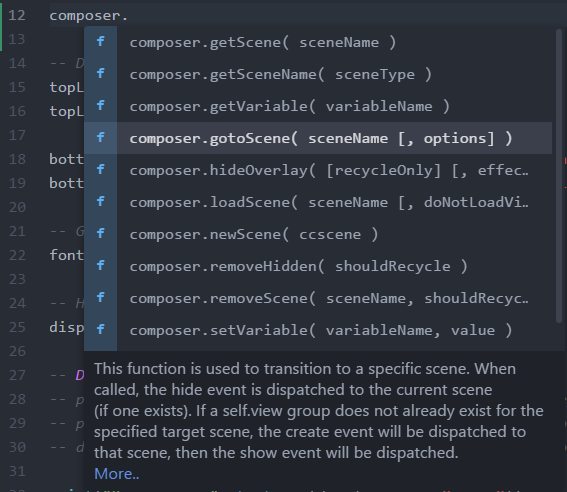
\includegraphics[width=0.9\textwidth]{img/atomPlugin}
				\caption{Il blando aiuto offerto dal plugin Corona per Atom}
				\label{fig:atomPlugin}
			\end{figure}
		
		\subsection{Build}
			
	
	
	\subsection{Usabilità}
	
		\paragraph{Menu}
		
		Pulsanti grandi per raggiungere facilitare la corretta pressione (44px).
		Il menu è situato sulla parte centrale dello schermo ossia la zona più facilmente accessibile per l'utente.
		
		A seguito della scarsa libreria \verb|widget| è compito veramente arduo andare incontro alla User Experience per progettare un'interfaccia originale e allo stesso tempo usabile. 
		
		Icone intuitive per il menu di gioco.
		
		Ogni sotto menu presenta il pulsante BACK il quale si trova al centro dello schermo e consente all'utente una veloce navigazione e esplorazione dei vari sotto menu.
		
		\paragraph{Gioco}
		Tutorial introduttivo che spiega come si gioca.
		
		Tutorial su misura che spiega i modi per mettere in pausa solo quando l'utente preme il pulsante pausa per la prima volta. In questo caso per testare l'uso dei sensori di Corona ho fatto sì che scuotere il device attivi la pausa.
		
		Il gioco funziona solo in posizione landscape left, in questo modo il pulsante di pausa del gioco nella versione Android non si trova vicino ai pulsanti di sistema.
		
		Il pulsante di pausa in gioco è situato in alto a sinistra, una zona
		
		

